%% main.tex
%%
%% This template requires IEEEtran.cls, written by Michael Shell, version
%% 1.7 or later.
%%
%% http://www.ieee.org/

\documentclass[conference]{IEEEtran}
\usepackage{graphicx}

\begin{document}

\title{A generic title}

\author{
\IEEEauthorblockN{Name}
\IEEEauthorblockA{
  Matter\\
  Location 1\\
  Location 2
}}

\maketitle

\begin{abstract}
  This is an abstract.
\end{abstract}

\section{Introduction}

This is an introductory section.

\section{Some Section 1}
\label{sec:section1}

Create a section and label it. You can also cite from the bibtex file: e.g.,
\cite{CaterSteel2006}, \cite{Abrahamsson2002}.

\begin{figure*}
	\centering
  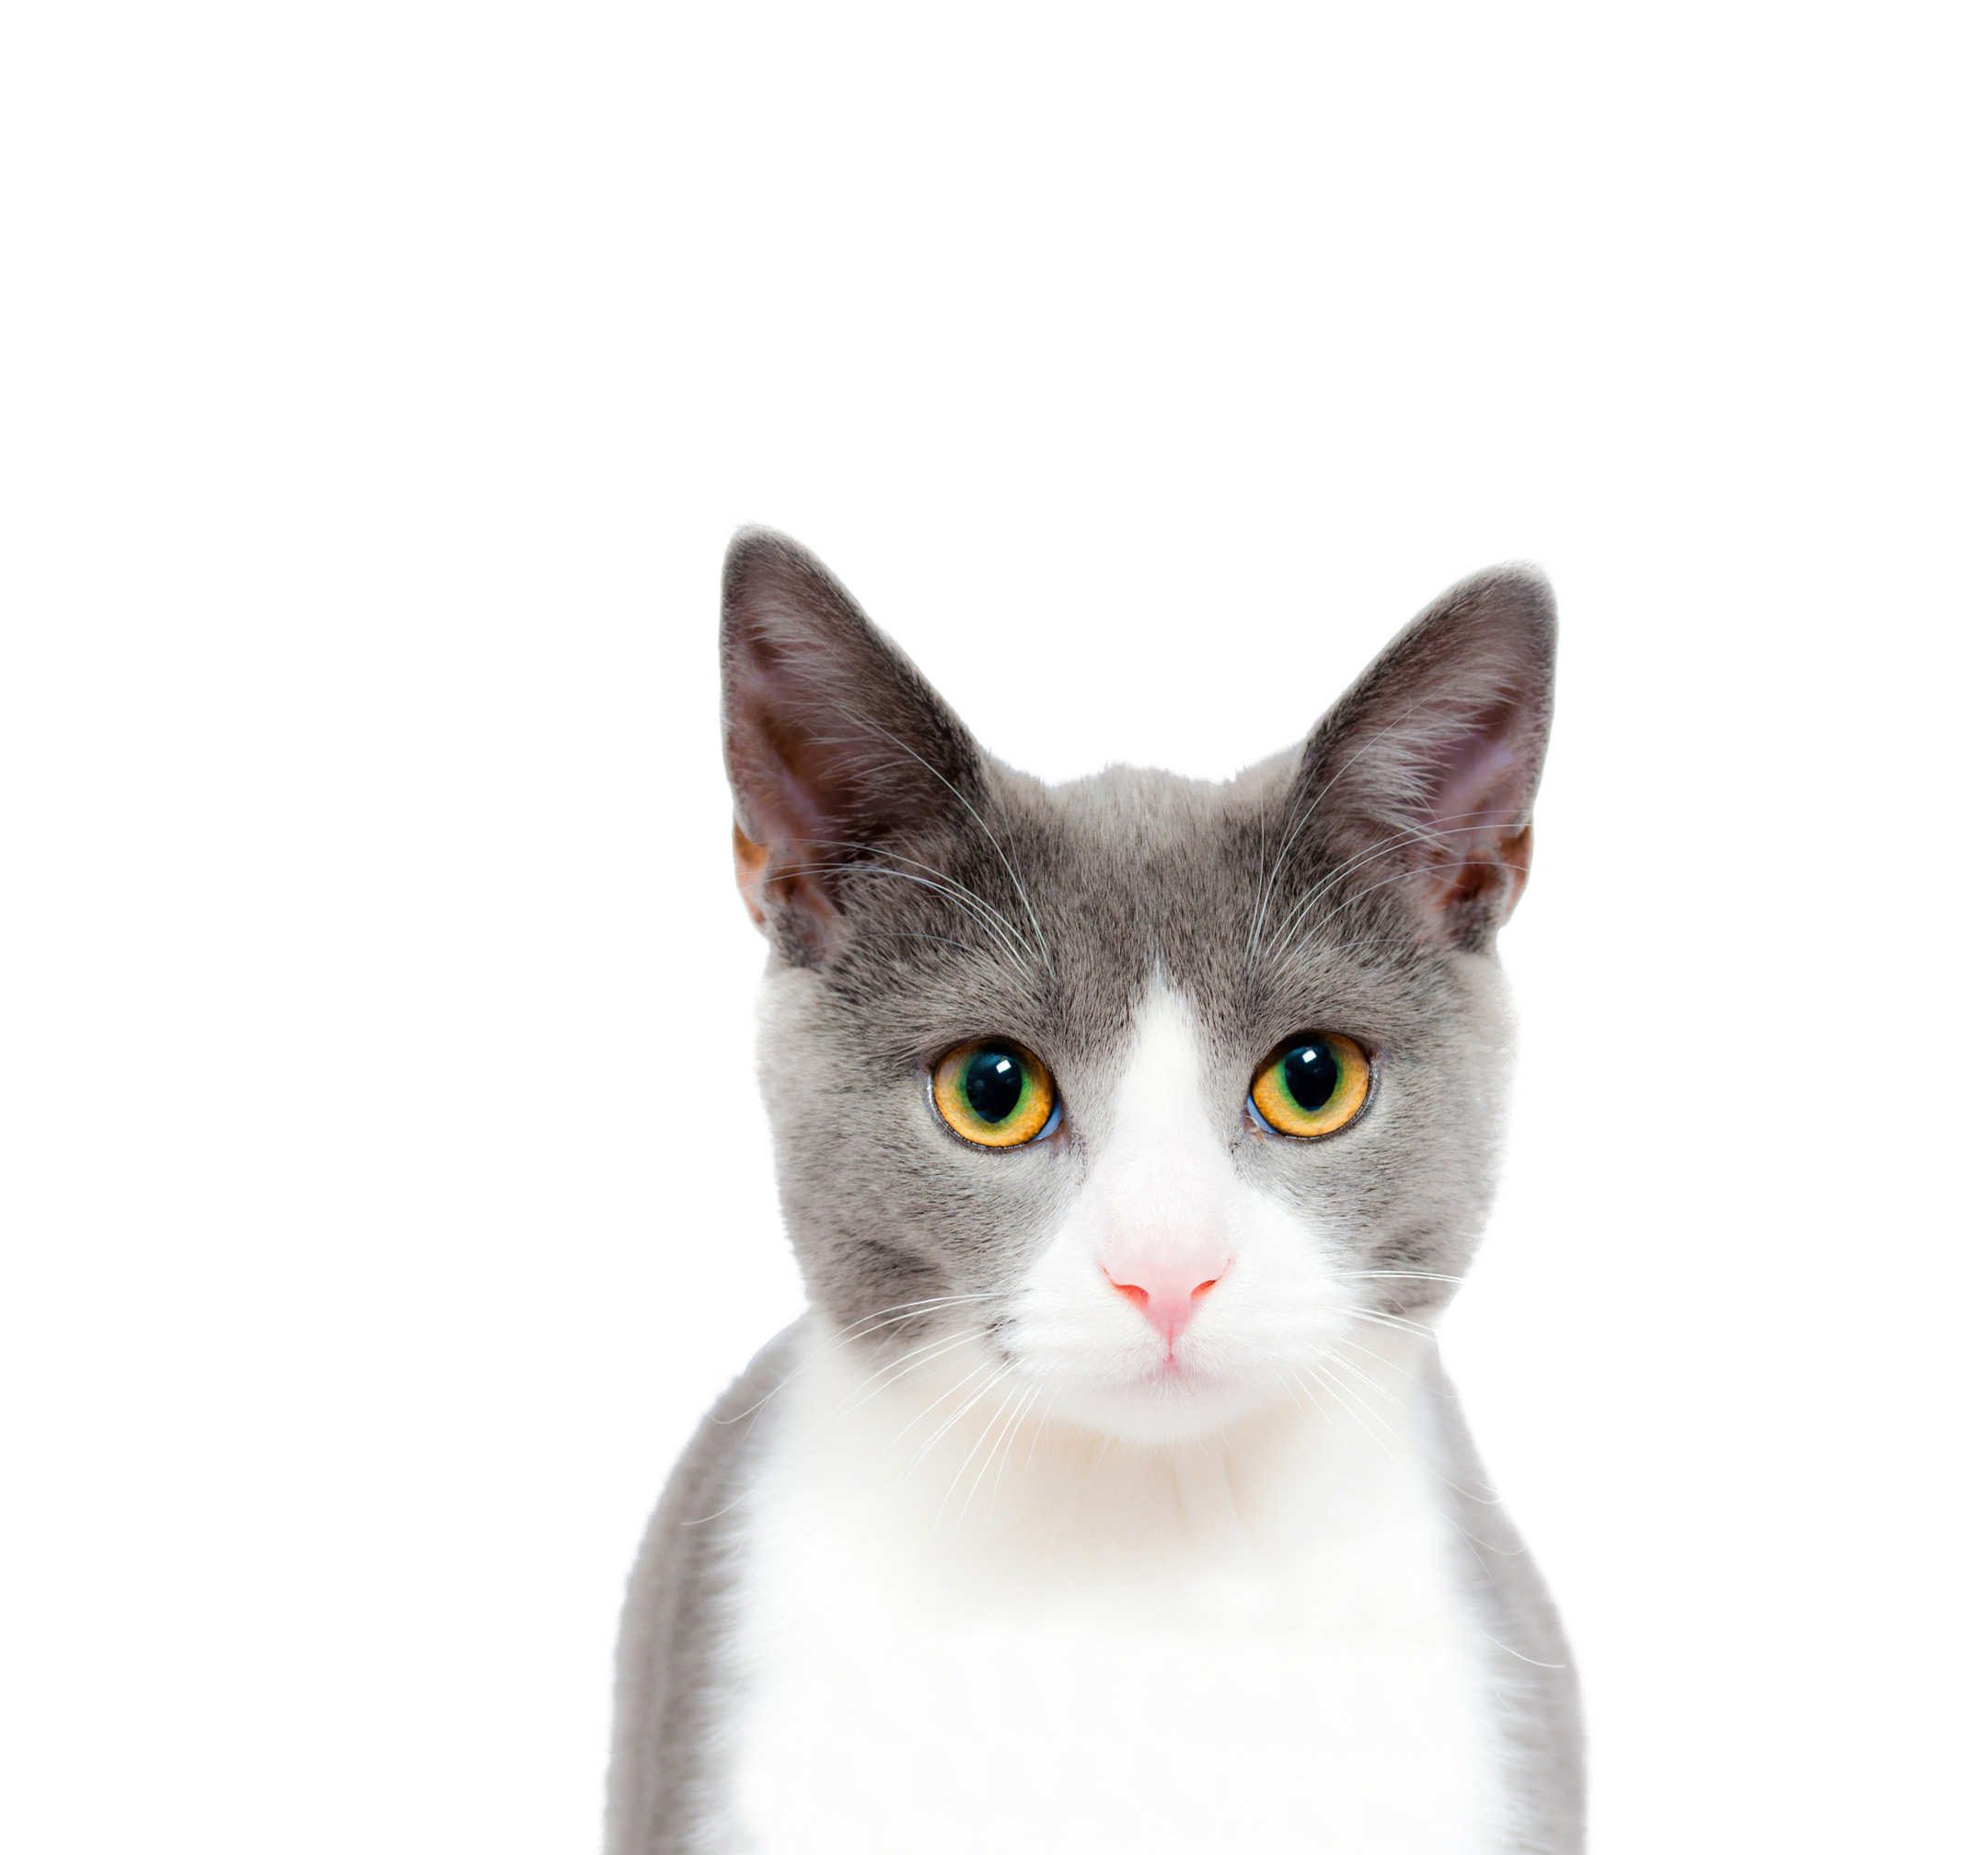
\includegraphics[width=0.9\textwidth]{template-pic}
	\caption{This is a caption}
	\label{fig:template-picture}
\end{figure*}

\section{Some section 2}
\label{sec:section2}

Yet another section, you can refer to other sections with ~\ref{sec:section1}.

% Generate the references section from the bib file.
\bibliographystyle{IEEEtran}
\bibliography{mybibfile}

\end{document}

%% EOF <<<<<<<<<<<<<<<<<<<<<<<<<<<<
